\begin{frame}
  \frametitle{Методы авторизации SSH. Ключи}

  \alert{Не хочешь вводить пароли?}
  \pause

  \alert{Не вводи!}
  \pause

  \begin{center}
    Aвторизация в SSH.

    Пара: открытый + секретный ключ.

    Вместо пароля.
  \end{center}

\end{frame}

\begin{frame}
  \frametitle{Ключи SSH. Создание}

  \begin{center}

    \begin{tabular}{ l r }
      \hbox{Linux: ssh-keygen} & \hbox{Windows: PuTTY keygen} \\
      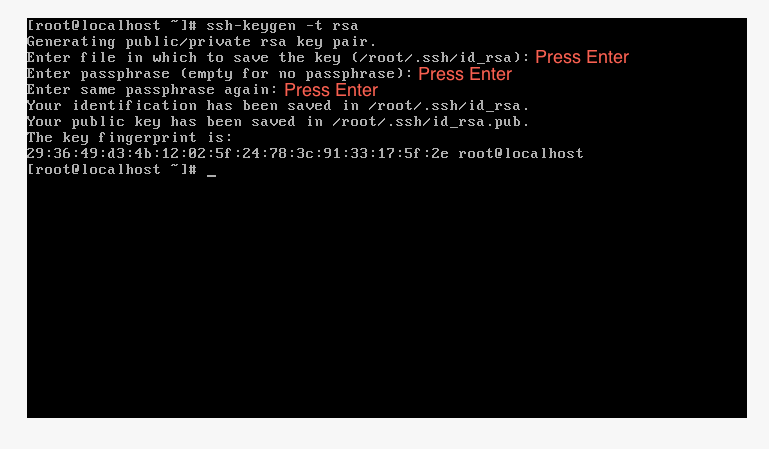
\includegraphics[height=3cm]{ssh-keygen-screenshot} & 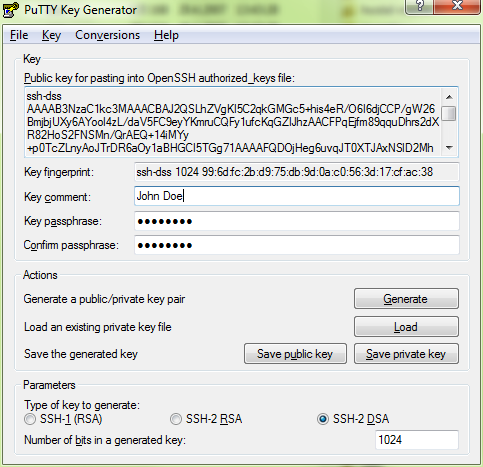
\includegraphics[height=4cm]{putty-keygen-screenshot} \\
      Ключи в папке .ssh/: & Ключи там, где сохранили \\
      id\_rsa и id\_rsa.pub &
    \end{tabular}

  \end{center}

\end{frame}


\begin{frame}
  \frametitle{Ключи SSH. Копирование}

  \begin{itemize}
    \item \alert{Что копировать?} Публичный ключ (id\_rsa.pub)  \pause
    \item \alert{Куда складывать?} в \$HOME/.ssh/authorized\_keys \newline удалённой машины \pause
    \item \alert{Как перенести?} \pause
      \begin{itemize}
        \item Linux: ssh-copy-id username@host \pause
        \item Copy-paste в редактор \pause
      \end{itemize}
  \end{itemize}

\end{frame}

\begin{frame}
\begin{columns}
    \begin{column}{0.5\textwidth}
      {\Large Linux: .ssh/config}
      \lstinputlisting[basicstyle=\tiny]{../../sam-solutions/samples/ssh-config} 
    \end{column}
    \begin{column}{0.5\textwidth}  %%<--- here
   {\Large Windows: PuTTY session}
        \begin{figure}
        \centering
            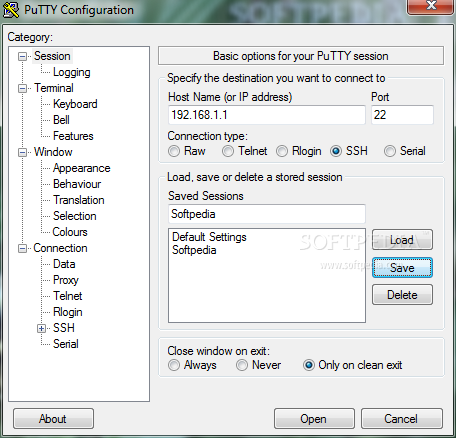
\includegraphics[scale=0.35]{putty-config-screenshot} 
        \end{figure}
    \end{column}
\end{columns}
\end{frame}
